\documentclass{article}

% Latex Tutorial beginners: http://www.latex-tutorial.com/tutorials/beginners/
\newcommand{\comment}[1]{}

\newcommand{\note}[1]{{\tiny (#1)}}

% Packages explained - Adding more functions to LATEX http://www.latex-tutorial.com/tutorials/beginners/lesson-3/
\usepackage[utf8]{inputenc}
\usepackage{booktabs}
\usepackage{url}
\usepackage{hyperref}
\usepackage{amsmath}
\usepackage{textgreek}
\usepackage{listings}
\usepackage{graphicx}
\usepackage[parfill]{parskip}
\usepackage[margin=1.3in]{geometry}

% fügt die Literatur auch zum Inhaltsverzeichnis hinzu (ist so nicht default)
\usepackage[nottoc,notlot,notlof,numbib]{tocbibind}

% Adding a bibliography http://www.latex-tutorial.com/tutorials/beginners/lesson-7/
\bibliographystyle{apalike}

\graphicspath{ {charts/} }
% Nested numbered enumerations, eg. 1.1, 1.2: http://tex.stackexchange.com/questions/78842/nested-enumeration-numbering
\renewcommand{\labelenumii}{\theenumii}
\renewcommand{\theenumii}{\theenumi.\arabic{enumii}.}


\title{
    Fitting Generalized Additive Models for\\ very large data sets with Apache Spark \\[7pt]
    \large Chapter Excerpt
}
\date{Future}
\author{Kai Thomas Brusch}

\begin{document}

    \pagenumbering{arabic}

    \maketitle

    \paragraph{Summary}

    This document contains three introductory chapters for my bachelor thesis titled "Fitting General Additive Models for very large datasets with Apache Spark".

    \paragraph{Contact} \texttt{kai.brusch@gmail.com}

    \paragraph{Location} Hochschule für Angewandte Wissenschaften Hamburg
    \paragraph{Department} Dept. Informatik
    \paragraph{Examiner} Prof. Dr. Michael Köhler-Bußmeier
    \paragraph{Second examiner} Dipl.-Mathematiker Univ. Markus Schmaus

    \newpage

    \tableofcontents

    \newpage

    
        \section{Statistical Learning}
    
    The topic of statistical learning might be alien to most computer science undergraduates. Thus, this first section is dedicated to introducing the area along with its problems and naming conventions \cite{hastie} describes Statistical learning as a set of tools for modeling and understanding complex data sets. Recent developments in statistics and computer science have created an interesting field that empowers modern statistical  with powerful computational methods. Statistical learning gives us the ability to ask interesting questions and use to data to find answers. This thesis will focus on one method of the supervised learning branch of statistical learning. Supervised learning methods build a statistical model for predictions and estimations of an output variable based on one or many input variables. Statistical learning methods are a cornerstone of modern scientific research and have given powerful methods to physics, neuroscience, biology, economics and every other relevant science. The professional world has been raving about the potential of statistical learning giving birth terms such as: Data Science and Big Data.
    
        \subsection{Why statistical learning?}
    
    Ideas are sometimes best conveyed through example. \cite{hastie} illustrated the benefits of statistical learning on a simple yet illustrative example. In the example we assume the be working for as statistical consultant in charge of advising a client on how to improve the sales of a given product. The client provides us with a data set containing the sales of a given product across several markets along with the budged for the product in each market in three different media outlets: TV, radio and newspaper. The client is not able to directly impact the amount of sales but he has the ability to change amount spend on each media outlet. If we can understand the number of items sold as a function of spend on media we can suggest our client to adjust spending to increase units sold. In \ref{fig:sales} the sales are plotted on the Y axis and the budget for a media outlet on the X axis. \ref{hastie} uses this example to introduce very important terminology. The media budgets are the input variable and sales are the output variables. The input variables are commonly denoted with $X_i$, in example $X_1$ is the TV spend, $X_2$ the radio spend and $X_3$ the newspaper spend. The naming for input variables has become inconsistent the the terms predictor, independent variables and features can be used interchangeably. The output variable, in this example the sales, is also called the response or dependant variable and denoted with Y.
    
        \begin{figure}
            \centering
            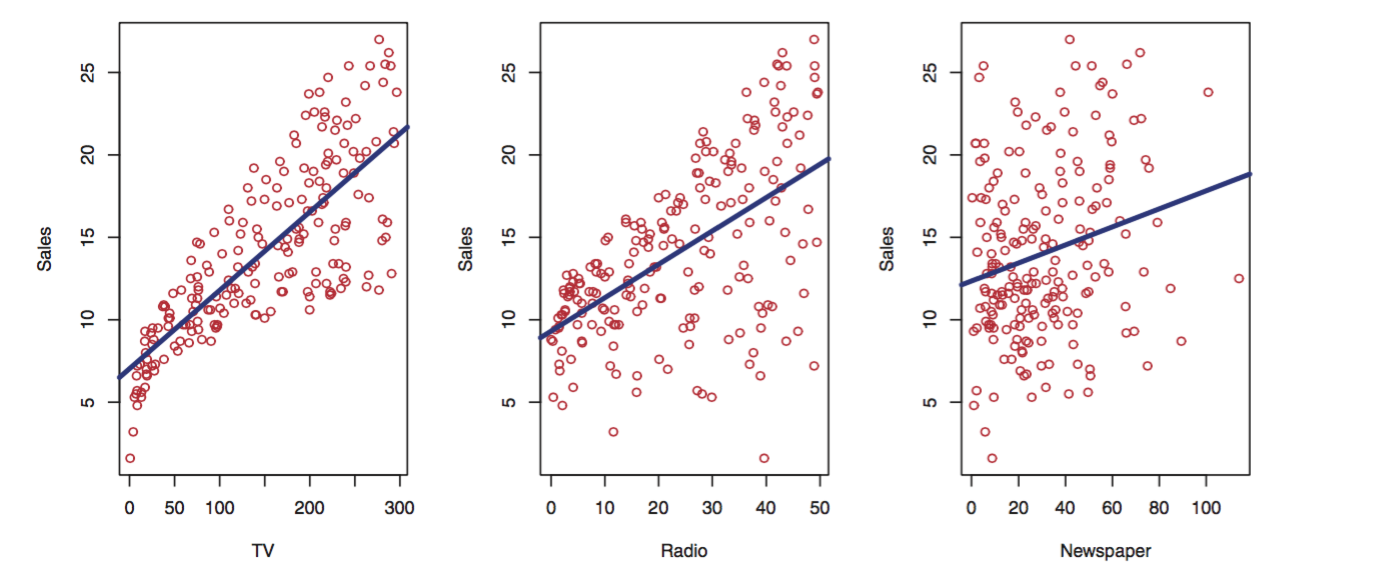
\includegraphics[width=\textwidth]{sales}
            \caption{We illustrate the units sold as a function of spend on each of the advertisement channels. The blue line is a linear model describing the underlying relationship between units sold and spend on media outlet.}
            \label{fig:sales}
        \end{figure}
        
    To generalize our sales example we can state the essential question of statistical learning. Supposed we observe a quantitative response Y and several predictors $X_1, X_2 , ... X_i$ we are looking for a relationship $f()$ that describes the relationship in the following form:
    \begin{equation}
        Y = f(X) + \epsilon
    \end{equation}
    The function $f()$ is a fixed but unknown function of the input variables $X_1, ... X_p$. $\epsilon$ is random, identical, independent distributed error term with zero mean. Another way of framing this is to see the function $f()$ as the systematic information in the observations. All statistical learning methods are concerned with finding an optimal $f()$. This thesis will introduce three, related methods of finding $f()$. Each with different idea on how to find $f()$ and with a different interpretation what optimal means.


    \subsection{Why Estimate f()?}
    While the example in the previous section showed statistical learning as a powerful tool to discover a relationship between a dependent and independent variable we have not explained why do we are keen to find a function $f()$. \cite{hastie} argues two essential reasons for estimating $f()$: inference and prediction. Inference is concerned with understanding a system while prediction wants to use the system to predict $Y$ on different values for $X$.
    
    Once a function $f()$ has been estimated on a given data set we can use that function to predict the value of Y for different $X_1 , ... ,X_p$. Predicting the value of Y new X values can be simple when the error term averages to zero. The value of Y can computed with the following equation:
    
    \begin{equation}
        \widehat{Y} = \widehat{f}(X)
    \end{equation}
    
    The wide hat notation stands for an approximation of an unknown value. $\widehat{f}$ is the estimated function for the true, unknown relationship $f()$ and $\widehat{Y}$ is an estimation of Y. The accuracy of our predicted $\widehat{Y}$ depends on two quantities: the reducible error and the irreducible error. The reducible error yields from the approximating nature of $\widehat{f()}$. The choice of $\widehat{f}$ causes the reducible error, a different approximation can change the reducible error. However, some of the error will always be unexplained and inherent in the measurements taken. This implicit error in our measurement can not be reduced and is thus called the irreducible error. \cite{hastie} formally describes the two types of error as
    \begin{equation}
        E(Y-\widehat{Y}) = E[f(X)+\epsilon - \widehat{f}(X)]^2 = [f(X)-\widehat{f}(X)] + Var(\epsilon)
    \end{equation}
    
    With $Var(\epsilon)$ being the irreducible error and $[f(X)-\widehat{f}(X)]$ the reducible part. Estimating $f$ to reduce the reducible error stands at the heart of statistical learning, the irreducible error can not be neglected however. The irreducible error is only assumed to be zero mean sum on the easiest of models, an important feature of models introduced later in this thesis is the assumption that the irreducible is in fact not zero sum average. 

    
    While prediction is focused on the looking forward, inference is the analytical perspective of statistical learning. Inference focuses on analysing the estimated $\widehat{f}$. Examining the respective contribution of each $X_1, ... , X_p$ to $Y$ can give qualitative insight into finding the best predictors $Y$ our of many. Returning to the previous example of budget spend on a media outlet. In \ref{fig:sales} we see that the number of sales respond differently to additional spend for each media category. Comparing the different $X$s we see that TV is by far the most efficient place to spend the budget. This simple analysis illustrates the power of inference to understand the underlying system. Understanding the basic nature of $X$'s influence on $Y$ is a key aspect of inference, does $Y$ in- or decrease with a change in $X$.  Inference further examines the fit of the function, \ref{fig:sales} assumes a linear relationship between each $X$ and $Y$, while this tread works well for TV it fails to capture the nature of the Newspaper category. A linear relationship between sales and Newspaper seems unreasonable after examination.   
    

     
    \subsection{How to estimate f()?}
    There are many approaches to estimate an unknown function given data points. \cite{hastie} states that all share certain characteristics. First all methods need training set of data. This training set contains tuples of dependant and independant variables. This set of tuples is used as input for an algorithm that approximates function $\widehat{f}()$. The methods for finding $\widehat{f}()$ can broadly be categories into two categories: parametric and non-parametric.
    
    Parametric models assume a specific shape of the true underlying function $f()$. This assumptions manifests itself in the two step approach to to parametric models, first make an assumption about the functional form or shape of f. The simples assumption and subject of the next chapter is the linear model. A linear assumption results in the following form:
    
    \begin{equation}
        f(X) = \beta_0 + \beta_1 X_1 + ... + \beta_p X_p
    \end{equation}
    
    The function f is linear in the influence of the parameter $\beta$. The linear assumption poses tight restrictions of the shape $f$ but also on space of potential functions. While a non-parametric function implies a search in an arbitrary p-dimensional function space the linear assumption limits the search to p+1 coefficients, $\beta_0,\beta_1, ... ,\beta_p$ in this example. 
    
    After deciding on shape for $f()$ the function needs to be estimated. The process of actually finding $f$ is also referred to as training or fitting a function. In this example this means fitting means to find the coefficients $\beta_0,\beta_1, ... ,\beta_p$. Thus the full problem of fitting a linear model becomes:
    
    \begin{equation}
        Y \approx \beta_0 + \beta_1 X_1 + ... + \beta_p X_p
    \end{equation}
    
    
    The shape decided in step one does not imply a method of actually finding the coefficients though there are best practices associated with each. The linear assumption in this example is mostly fit with a least squares method which again can be computer with different methods. So the choice of a parametric form solely dictated the nature and number of the parameters involved, thus the name: parametric.
    
    Choosing a functional shape for $f()$ drastically simplifies the fitting process by predetermining the amount of coefficients to be estimated. The chosen shape may however enforce conditions that are very different to the original function f. A poor choice of the parametric form will directly translate into a poor estimate. This problem can be addressed with more flexible methods that allow for a more parameters. The higher number of parameters has to be carefully weighed with a phenomena called over fitting. Over fitting is the result of giving a functional form too many parameters, causing the approximation to follow the error too closely. A major benefit of parametric methods is the ability to interpret the results. Assuming a functional shape usually yields from information about the function that is not in the data itself. Accounting for outside information though a choice of parametric shape allows for an easy interpret ability as the result must fit the picked framework.
    
    \cite{hastie} describes the non-parametric approach as the complement to the parametric methods. Non-parametric methods do not assume the functional form of $f$ before estimating it. This brings a major advantage over parametric methods since they allows $f$ to follow the data as closely as possible without dealing with a determined shape. Allowing $f$ to take any arbitrary form is a large advantage and offers much more flexibility then parametric methods. While non-parametric methods avoid the pitfall of  a bad functional shape they don't reduce the space of f by predetermining the number of coefficients. Non-parametric methods provide much more flexibility than parametric methods and are usually preferred for prediction. Their arbitrary results makes the interpretation of the result harder to understand and are a clear disadvantages over parametric methods.
    
    The method central to this thesis follows a progression through the parametric, non-parametric framework. The simple linear model will be the first model introduced and is a parametric method. The linear model assumes a linear relationship between $X$ and $Y$ which makes it the easiest to estimate and interpret. Enforcing very strict limitations on functional form, only allowing a linear relationship with a normal distributed response variable and a zero mean error term. The generalized linear model extends the linear model by easing the restriction on the response variable and allowing for a varying error term. Even though the restrictions on the functional shape are eased in the generalized linear model they are still a parametric methods with all the advantages and disadvantages. Generalized additive models stand at the heart of the thesis and present an interesting extension of the generalized linear model. Generalized additive models allow for a non-parametric method called splines to be used as part of generalized linear models. Splines are a highly flexible non-parametric method that allow to fit arbitrary functions. Generalized additive models offer much greater flexibility than generalized linear models but rely on similar estimation technique and theory. This progression with an implementation of generalized additive models in a cluster environment will be the central piece of this thesis.
    
    
    \subsection{Statistical Computing Environment: R}
        
    R is a free software environment for statistical computing and graphics. R is designed to express statistical models and comes with an development environment that is build to illustrate and discover data.   
        
    
    
    \section{Generalized Linear Models}
        \subsection{Linear Model}
        \subsubsection{Least Squares}
        \subsubsection{Linear Model Example }
        \subsection{Generalized Linear Model}
        \subsubsection{Iterative Reweighted Least Squares}
        \subsubsection{Generalized Linear Model Example}
    
    \section{Generalized Additive Models}
        \subsection{Regression Splines}
            \subsubsection{Basis Functions}
            \subsubsection{Cyclic Cubic Regression Splines}
        \subsection{Penalized Iterative Reweighted Least Squares}
        \subsection{Generalized Additive Models Example}
        \subsection{Numerical Optimizations For Large Data Sets}
    
    \section{Apache Spark}
        \subsection{General In Memory Cluster Computing Framework}
        \subsection{The Language Scala and Breeze}
        \subsection{Machine Learning Pipeline}
        \subsection{Implementing Generalized Additve Models in Apache Spark}
    
    \section{Matrix Algebra Apendix}
        \subsection{QR Decomposition}
        
    


    \newpage

    \bibliography{thesis}    % reference to thesis.bib

    \newpage

\end{document}
